
\section{Convolutional Neural Networks}\label{sec:cnn}

As discussed in the previous sections, both K-means clustering and SAM struggle to reliably distinguish between oxidation and coating layers in complex samples.

Convolutional Neural Networks (CNNs) \cite{oshea_introduction_2015} offer a promising alternative. CNNs are supervised machine learning models that are well-suited for image-related tasks, especially where the spatial relationships between pixels are important. This makes them a good candidate for solving segmentation problems in images where traditional methods fail. An important advantage of CNNs is that they can be trained specifically on the dataset used in this project, with the ability to adapt to the particular features of the coating and oxidation layers. They also require less computational power than SAM, making them more suitable.

However, CNNs require ground truth labels for training, which were not initially available.

As mentioned in Section~\ref{sec:ManualProc}, the only available data were microscope images and an Excel spreadsheet with length of the expert-made measurmenrs. Unfortunately, this was not enough to fully reconstruct the original measurements. Since labeling all data manually would have been too time-consuming, three alternative strategies for dataset creation were explored.

First, a few small adjustments were made to the labeling tool Fiji, to allow researchers to create data that could later be converted into 2D polygon labels. While researchers were labeling the initial set of samples to obtain a reasonable dataset, two additional approaches were explored in parallel.

The first approach was to reuse the K-means segmentation results from previous experiment. The second approach involved manually refining the K-means labels in collaboration with researchers to create high-quality ground truth labels. These refined labels are especially important, as they represent the most accurate annotations available and are used for evaluation on the test set.



\subsection{Fiji Adjustments}\label{sec:1.2.2}

The whole manual labeling is done in Fiji. To make the data collection possible, a few important adjustments were made. The adjustments involved the customization of the `StartUpMacro` in Fiji, which runs automatically each time the program is launched. Three new buttons were incorporated into the interface: one for saving measurements, another for adjusting the scale, and a third for displaying the default lines, which represent the default expert-made measurements.

The \texttt{Save Measurement} button was implemented to store data from the 20 lines required to create the dataset. This feature ensures that the required measurements are automatically saved.

The \texttt{Adjust Scale} button was added to streamline user interaction with Fiji, addressing the need to manually adjust the scale at the start of each session. Since the scale, visible at the bottom of the image, remains constant across all images, this functionality simplifies the process.

The \texttt{Set Default Lines} button was introduced to allow the researcher to quickly access the prepared default 20 lines for the new set.

Furthermore, the extraction of the final measured lengths into an Excel file was simplified.

\subsection{Types of Labels}\label{sec:masks}


The following three sections present strategies of label creation mentioned in ~\ref{sec:cnn} in more detail.



\subsubsection{Polygon labels}

This set of labels was generated using measured data from expert-made measurements. The upper ten points of each line were connected to form a boundary curve, and the same process was applied to the lower points. The space between these two curves was then filled to generate the label. However, due to missing information at the edges of the image, cropping of both the images and the labels was needed. Figures~\ref{fig:polygon_sem_color} illustrate that the labels do not extend to the edges of the images. While these labels are not highly precise, their creation process is highly efficient, focusing on the 20 key points defined by the researcher. Due to their efficiency, they are considered valuable for testing in the training process, as they provide a balance between accuracy and computational effort.



Linear interpolation was employed to connect the boundary points. The upper and lower boundary points, stored in arrays, created a boundary curve by connecting each pair of neighboring expert-made measurement points with a straight line. The region between the interpolated upper and lower curves was then filled, resulting in a binary label. 

Linear interpolation involves estimating values between two known points. It assumes a linear relationship and is defined by the following equation:

\begin{equation}
y(x) = y_1 + \frac{(x - x_1)}{(x_2 - x_1)} (y_2 - y_1)
\end{equation}

Here, $(x_1, y_1)$ and $(x_2, y_2)$ are two neighboring known points, and $y(x)$ represents the interpolated value at a given $x$ such that $x_1 \leq x \leq x_2$. 

This approach enabled the automated generation of labels from the measured lines, ensuring that the labels were consistent with the scientific data.



\subsubsection{K-means labels} \label{sec:means_mask
}


Despite these limitations mentioned in Section~\ref{fig:kmean}, the labels generated by the K-means algorithm were still used to create a second dataset. This approach was faster than expert-made manual measurements and, in many cases, provided a more precise boundary for the coating layer—something the polygon labels couldn't offer. However, one downside was that the oxidation areas were often grouped with the coating layer due to their similar pixel values. This can introduce noise into the data, potentially affecting the model’s ability to generalize.
\subsubsection{K-means Refined}


To improve the accuracy of the K-means labels, the entire dataset was reviewed in collaboration with the researcher, and the labels were manually refined using image editing software. Additionally, the manual revision process was much less time-consuming than the complete manual annotation of every image, due to the predefined labels from K-means. The final version of these labels was then used as a test dataset for further automation. This label is shown in Figure~\ref{fig:3}.


\begin{figure}[H]
    \centering

    % First row
    \begin{subfigure}{0.8\textwidth}
        \centering
        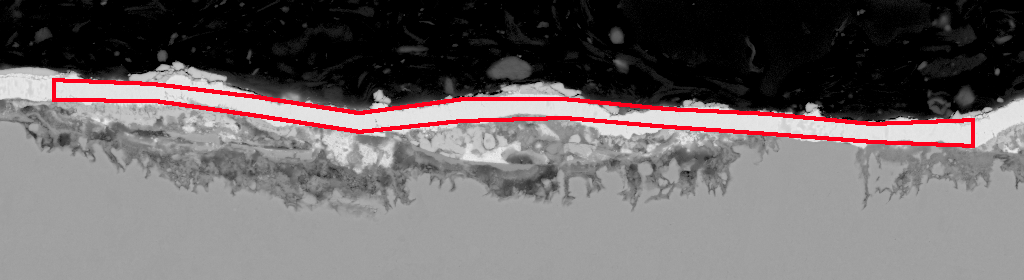
\includegraphics[width=\linewidth]{PICTURES/MASK/2.png}
        \caption{Polygon label}
        \label{fig:polygon_sem_color}
    \end{subfigure}

    \begin{subfigure}{0.8\textwidth}
        \centering
        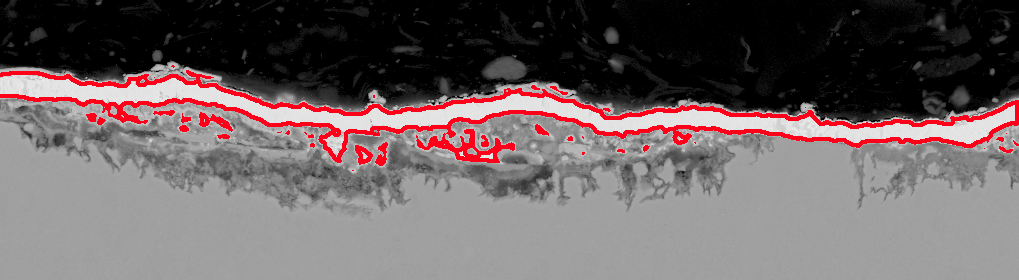
\includegraphics[width=\linewidth]{PICTURES/MASK/1.png}
        \caption{K-Means label}
        \label{fig:kmean_sem_color}
    \end{subfigure}

    \begin{subfigure}{0.8\textwidth}
        \centering
        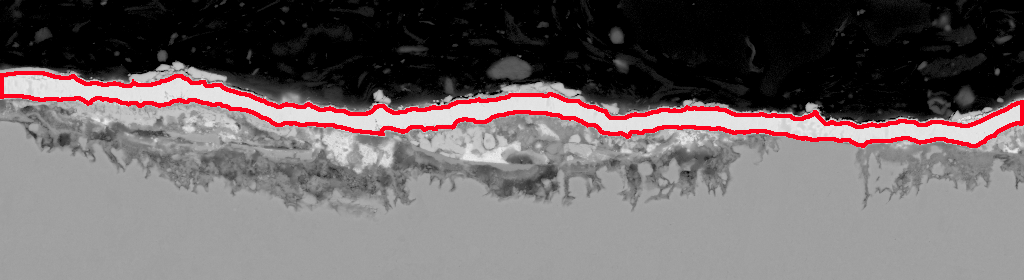
\includegraphics[width=\linewidth]{PICTURES/MASK/3.png}
        \caption{Refined K-Means label}
        \label{fig:3}
    \end{subfigure}

    \caption{Examples of polygon, K-Means, and refined K-Means labels, shown as red-highlighted borders over the original SEM image.}    \label{fig:all-masks}
\end{figure}

%As discussed in the previous section, K-Means clustering struggled to distinguish between the oxidation and coating layers in complex samples. Figure~\ref{fig:149} demonstrates the predicted mask generated by training the CNN model, which successfully segments the coating layer. In contrast, Figure~\ref{fig:kmean_sem_color} illustrates the coating segmentation using the K-means algorithm, highlighting its limitations in separating the two segments.

\subsection{U-Net Architecture}

After collecting the entire dataset, a suitable CNN architecture needed to be selected. For this task, the U-Net architecture\cite{ronneberger2015unetconvolutionalnetworksbiomedical} is particularly effective. U-Net has shown strong performance in various segmentation problems, especially in biomedical imaging. Unlike typical CNNs used for classification, U-Net is designed for pixel-wise classification, making it ideal for tasks requiring precise localization of objects, such as in microscopy images. The U-Net architecture consists of two main components:

\begin{itemize}
    \item \textbf{Contracting path (Encoder)}: The left side of the U-Net includes a series of convolutional, activation, and pooling layers that progressively reduce the image's dimensions. This part extracts features from the input image.
    
    \item \textbf{Expanding path (Decoder)}: The right side of the U-Net gradually upsamples the feature maps back to the original image size. This step recovers spatial resolution lost during downsampling and ensures precise pixel-wise segmentation.
\end{itemize}

\begin{figure}[H]
    \centering
    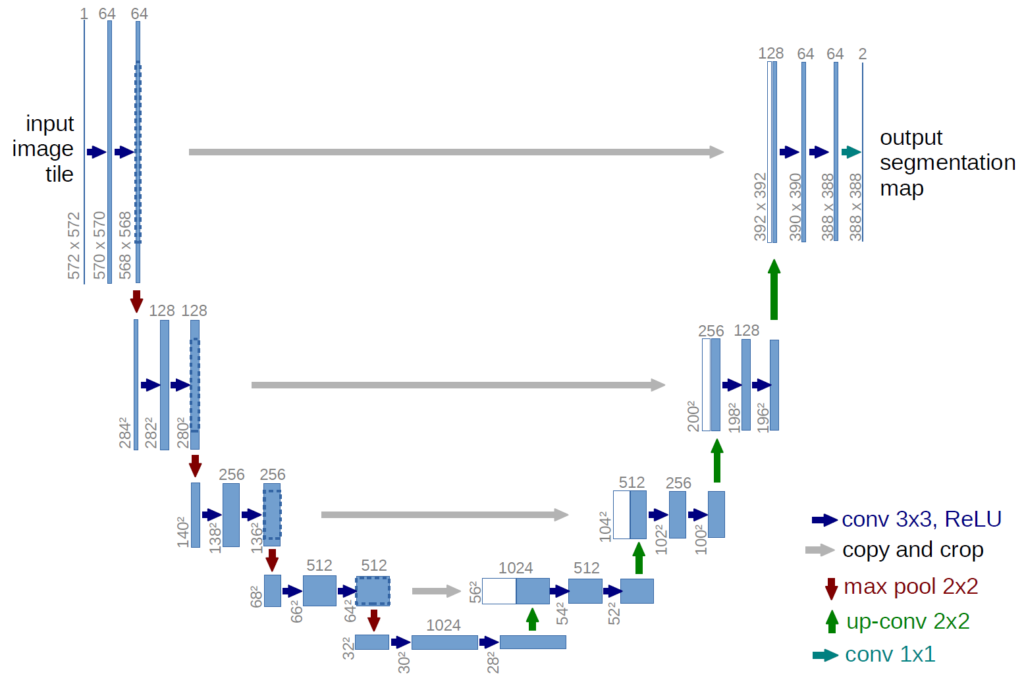
\includegraphics[width=0.8\linewidth]{PICTURES/unet-architecture.png}
    \caption{U-Net architecture \cite{ronneberger_u-net_2015}}
    \label{fig:unet-architecture}
\end{figure}

The input to a U-Net model is typically an image of size $H \times W \times C$, where $H$ is the height, $W$ is the width, and $C$ is the number of input channels. In Figure~\ref{fig:unet-architecture}, the input consists of grayscale images, where $C = 1$. For RGB images, $C = 3$. The output is an image of size $H \times W \times N$, where $N$ is the number of segmentation classes. In this case, there are two classes (binary segmentation), so $N = 2$.

\subsubsection{Upsampling with Transpose Convolutions}

The expanding path uses transpose convolutions (also called deconvolutions). Convolution reduces the image to a feature map, while transpose convolution upsamples the feature map back into an image.

\subsubsection{Skip Connections}

During the downsampling process, the network learns various features. However, as the feature maps shrink, details are lost. Skip connections allow the network to preserve these details by carrying them over from the earlier layers in the contracting path to the corresponding layers in the expanding path. This process helps retain important spatial information, improving segmentation accuracy. These connections are represented by the horizontal arrows in Figure~\ref{fig:unet-architecture}.
\subsubsection{Key Steps in U-Net Processing}
\begin{enumerate}
    \item In the contracting path, feature maps are progressively downsampled until the lowest resolution is reached.
    \item Before each downsampling step, feature maps are saved.
    \item During the upsampling process, saved feature maps are combined with the upsampled maps to recover spatial details \cite{ronneberger_u-net_2015}.
\end{enumerate}

\subsection{U-net and Microscopy}
A 2023 survey \cite{wu_state---art_2024} highlights U-Net as an effective model for microscopic image segmentation. This success is attributed to its ability to perform well with limited training data and its relatively quick training process. The survey also emphasizes the use of the original, unmodified U-Net, which has been widely applied in fields such as cytology and geology \cite{chen_deep_2020} (e.g., using scanning electron microscopy). Given that the images in this dataset share similar characteristics, the U-Net architecture is considered suitable for this task.

\subsection{Data Preprocessing – Augmentation} \label{sec:aug}
The dataset consists of 130 training images, which are divided into training and validation subsets in a 75:25 ratio, along with 47 test images. Because of the limited data, augmentation is applied to the training set to better showcase potential deviations in visual representation. Thus, the model can learn to generalize better to variations it might encounter during future prediction. 

The first step involves either cropping or resizing the image to a size of $(n \times 1.5) \times (n \times 1.5)$, with equal probability, where $n$ is the patch size and a model hyperparameter. Cropping keeps the original resolution, while resizing includes more context to reduce overfitting. Cropping is done using the \textit{CropNonEmptyMaskIfExists} function \cite{info11020125}, ensuring the region contains part of the coating. After additional augmentations, the image is cropped to a final size of $n \times n$ to match the model input.

Additional augmentations include:

\begin{itemize}
    \item \textbf{Brightness and contrast adjustment:}This simulates lighting variations.
    \item \textbf{Sharpening:} This enhances the details in the image.
    \item \textbf{Horizontal flipping:} The image is mirrored along the horizontal axis to reduce positional bias.
    \item \textbf{Elastic transformation:} A non-linear deformation is applied to simulate distortions and improve generalization.
    \item \textbf{Rotation:} The image is rotated randomly within the range of -90° to 90° to simulate different orientations.
\end{itemize}

The effects of these augmentations are illustrated in Figure \ref{fig:augmentation}, where different transformations are applied to a sample image.

\begin{figure}[H]
\centering
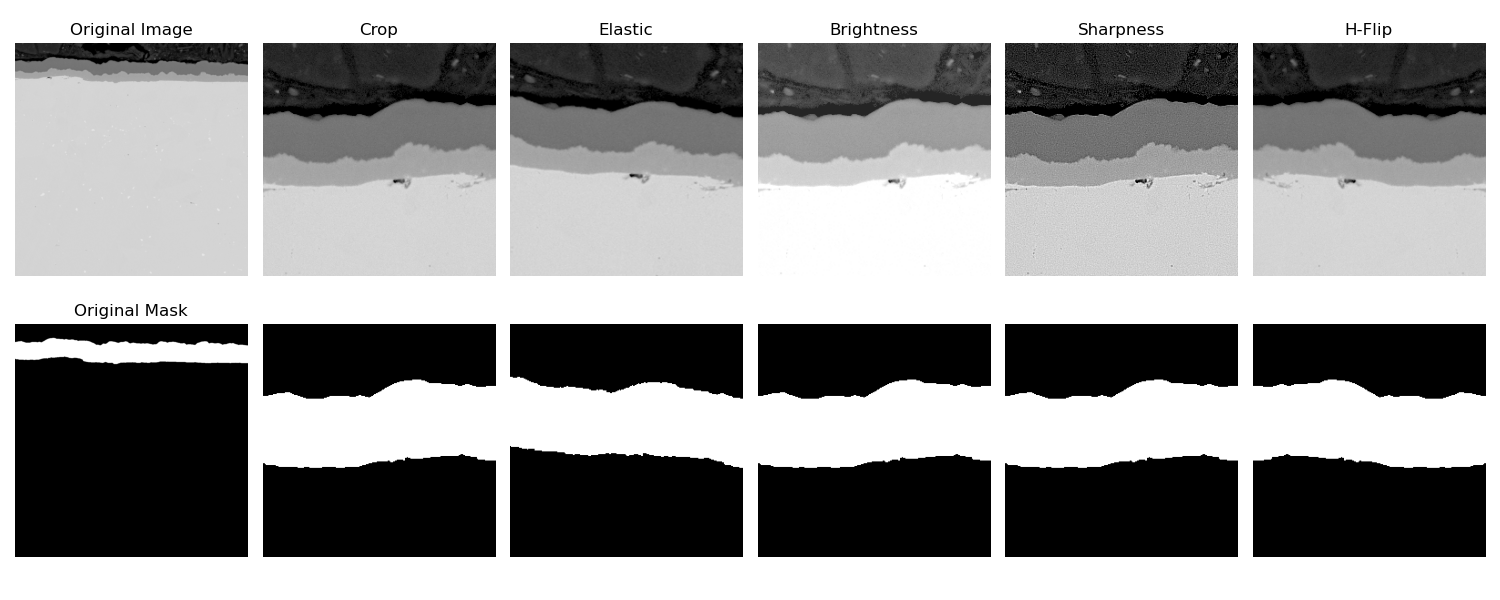
\includegraphics[width=1\linewidth]{PICTURES/augumentation.png}
\caption{Illustration of various augmentation techniques applied to the dataset.}
\label{fig:augmentation}
\end{figure}

\subsection{Technical Details}
The \texttt{segmentation\_models} library \cite{Iakubovskii:2019} was used for the U-Net implementation. Documentation for this implementation can be found \href{https://smp.readthedocs.io/en/latest/models.html#id22}{here}\cite{SegmentationModelsPyTorch}. After initializing the training functions and other helper functions, hyperparameter tuning can begin. The main hyperparameters include depth, patch\_size, filters, and learning rate, all of which will be tested.

\subsubsection{Depth}
The depth of a U-Net is determined by the number of encoder and decoder blocks. This influences the model's ability to capture features within the input image. For instance, in Figure~\ref{fig:unet-architecture}, the depth is 5.

A deeper network (higher depth) can handle complex data with high variability, but may suffer from excessive downsampling and overfitting. In contrast, a shallower network may struggle to extract relevant features and differentiate between noise and useful information.

\subsubsection{Patch Size}
Patch size plays a crucial role in how well the model learns different features from the image.

Smaller patches allow the model to focus on fine details but might miss the broader context, making it harder to understand relationships between different parts of the image.

Larger patches capture more context and larger structures, but may lose fine details.

To ensure that the region of interest, specifically the coating layer, is always included, the images are cropped in a way that retains this key feature.

\subsubsection{Filters}
The filters parameter determines the number of filters used in each encoder and decoder layer, which affects the number of feature maps generated by the model. In the code, the number of filters in the decoder is calculated as follows:

\begin{verbatim}
decoder_channels = [filters * 2**i for i in range(depth, 0, -1)]
\end{verbatim}

This calculation, inspired by the original U-Net architecture, doubles the number of filters at each downsampling step \cite{2018arXiv180906839B}. For example, with \texttt{filters = 8} and \texttt{depth = 3}, the number of filters would be:  
\\\textbf{Encoder:} 8, 16, 32 \\
\textbf{Decoder:} 32, 16, 8

Using more filters allows the model to learn more complex patterns. However, it can also increase the risk of overfitting when there is insufficient training data. On the other hand, using fewer filters might prevent the model from capturing important features, reducing its performance.
\subsubsection{Hyperparameter values}\label{sec:1.2.8}

In this project, all combinations of the following hyperparameters were tested:

\begin{itemize}
    \item \textbf{Patch size:} 128, 256
    \item \textbf{Depth:} 3, 4, 5
    \item \textbf{Filters:} 8, 16, 32
\end{itemize}

\subsection{Learning Rate and Schedulers}\label{sec:1.2.9}

During training, the model's parameters are adjusted to find the optimal solution. The \textbf{Adam optimizer} \cite{kingma2017adammethodstochasticoptimization} is used for this purpose. Adam (Adaptive Moment Estimation) calculates adaptive learning rates for each parameter.

Since Adam adapts the learning rate, manually modifying it can have a small impact but still affect performance. The learning rate is chosen from a range between 0 and the set value.

\begin{itemize}
    \item \textbf{Linear Scheduler:} The learning rate starts at the set value and decays linearly. The \textbf{end factor} multiplies the learning rate to finish at \textbf{end factor * lr}.
    \item \textbf{Warmup Cosine Scheduler:} The learning rate starts at a predefined value and decreases over \texttt{T\_0} epochs, following a cosine annealing schedule. After reaching the minimum, the learning rate resets and begins from the previous value, restarting the cycle.
\end{itemize}

The following schedulers and values were tested:
\begin{itemize}
    \item \textbf{LR values}: 0.01, 0.001, 0.0001
    \item \textbf{Linear scheduler}: With end factors of 0.01 and 0.001
    \item \textbf{Warmup Cosine scheduler}: With \texttt{T\_0}$= 25$ and \texttt{T\_0}$= 50$
\end{itemize}

Figure~\ref{fig:LRS} shows the learning rate schedulers. On the left, the linear scheduler spans 200 epochs, starting at 0.01 and ending at 0.001. On the right, the warmup cosine scheduler starts at 0.01 and ends at 0.00, with a warmup phase during the first 50 epochs.

\begin{figure}[H]
    \centering
    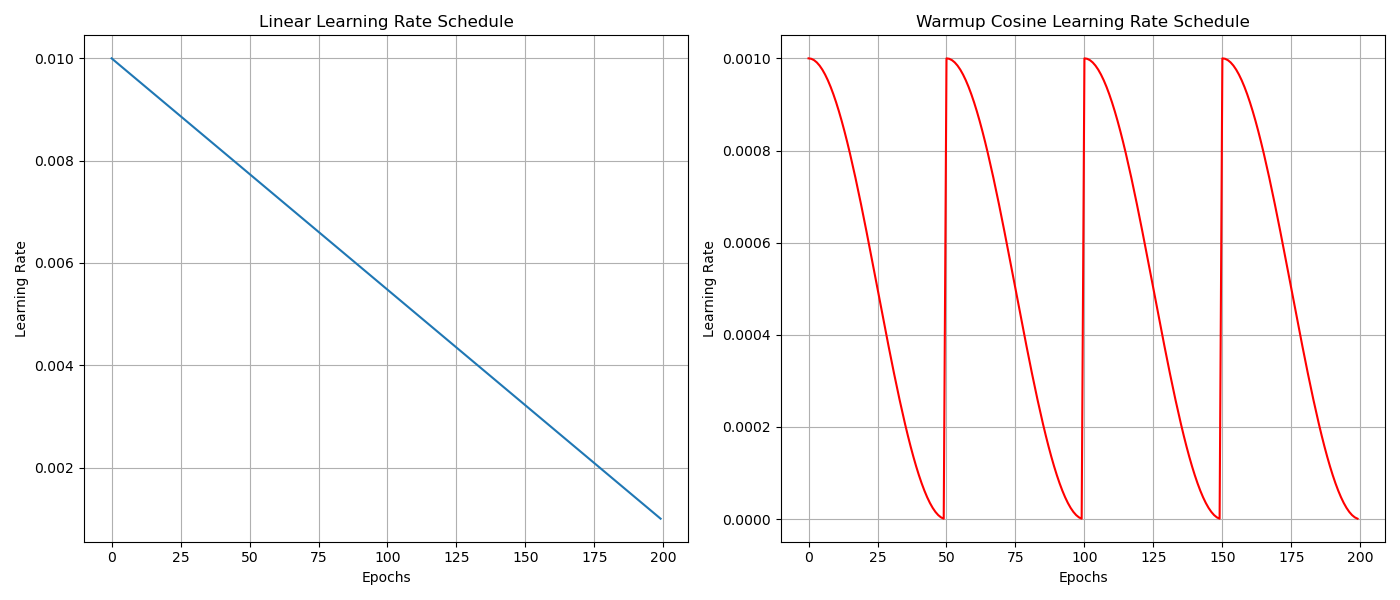
\includegraphics[width=0.9\linewidth]{PICTURES/LRS.png}
    \caption{Learning Rate Schedulers (LRS)}
    \label{fig:LRS}
\end{figure}
\subsection{Loss Function}\label{IoU}

The loss function \( L(Y, \hat{Y}) \) is used to evaluate prediction errors. Since the model's performance on test data is assessed using the Intersection over Union (IoU) metric, IoU is also used as the loss function during training and validation.

The IoU is defined as:

\begin{equation}
\text{IoU} = \frac{\text{intersection} + \text{smooth}}{\text{union} + \text{smooth}}
\label{eq:iou}
\end{equation}


Where:
\begin{itemize}
    \item The \( \text{intersection} \) is the number of pixels correctly predicted as the foreground (\(\text{True Positives}\)).
    \item The \( \text{union} \) consists of all pixels predicted or labeled as foreground. It equals the sum of \( \text{True Positives (TP)} \), \( \text{False Positives (FP)} \), and \( \text{False Negatives (FN)} \).
\end{itemize}

Thus, the IoU formula becomes:

\begin{equation}
\text{IoU} = \frac{\text{TP} + \text{smooth}}{\text{TP} + \text{FP} + \text{FN} + \text{smooth}}
\label{eq:iou_smooth}
\end{equation}


The smoothing constant (\(\text{smooth} = 1\)) prevents division by zero. The loss function returns \( 1 - \text{IoU} \), ensuring that lower values indicate better model performance.

\subsection{Training}

After defining the key components, model training begins. The dataset is divided into 98 training images and 32 validation images. The training, validation, and testing labels come from the K-means refined dataset, with the validation set remaining fixed as a single batch.

During training, just the training data are shuffled each epoch to reduce the risk of overfitting. The DataLoader then creates batches of 32 augmented images from the shuffled data. Training proceeds for 200 epochs, with each epoch consisting of both training and validation phases.

\subsubsection{Training Phase}

In each epoch, the training dataset is shuffled, and three batches of 32 images are formed. The model predicts the binary label for each batch and computes the training loss. Backpropagation adjusts the model's parameters using the optimizer based on the computed loss.

\subsubsection{Validation Phase}

At the end of each epoch, the validation set (a single batch) is evaluated using the loss function. The model's parameters are not updated during this phase. If the validation loss is lower than the previously recorded minimum, the model and its parameters are saved, and the minimum validation loss is updated.

\subsection{Optimization Strategy}

\begin{enumerate}
    \item Three optimization runs were performed to determine the optimal learning rate (LR) and learning rate scheduler. Details about the hyperparameters tested are provided in section \ref{sec:1.2.9}.
    \item The main optimization focused on the three key hyperparameters, using the best LR and LR scheduler from the initial optimization. The specific hyperparameters optimized are discussed in section \ref{sec:1.2.8}.
    \item After identifying the best hyperparameters, two additional runs were conducted. One used polygon labels, while the other used non-refined K-means labels.
\end{enumerate}
\subsection{Optimization results}

The optimization of the learning rate and learning rate schedulers is discussed first. The schedulers were tested with the hyperparameters \textbf{depth = 3}, \textbf{patch size = 128}, and \textbf{filters = 8}. These values were chosen as they offered the best computational efficiency among the tested ones. 

Table \ref{tab:scheduler_results} summarizes the best results for different learning rate schedulers. The linear scheduler achieved the lowest objective function value of 0.06429 with a learning rate of 0.001 and an end factor of 0.01. 

\begin{table}[H]
    \centering
    \caption{Best results for different Learning Rate Schedulers.}
    \begin{tabular}{lccc}
        \toprule
        Schedule & Learning Rate (lr) & End Factor / \( T_0 \) & Val Loss \\
        \midrule
        Warmup Cosine & 0.001 & 50 & 0.06527 \\
        Linear & 0.001 & 0.01 & 0.06429 \\
        None & 0.001 & --- &  0.06474 \\
        \bottomrule
    \end{tabular}
    \label{tab:scheduler_results}
\end{table}

It is evident that a learning rate of 0.001 consistently outperformed the others across all three optimization experiments. In contrast, the choice of scheduler did not lead to significant differences in the validation loss values, indicating that it had only a minor influence on the training process.

Figure~\ref{fig:loss-None} illustrates the validation loss progression over 200 epochs for three different learning rates, without the use of any learning rate scheduler. Trial 0, corresponding to a learning rate of 0.0001, shows a very stable but very slow decay in validation loss, suggesting that the learning rate is too low to enable efficient convergence. Trial 1, with a learning rate of 0.001, demonstrates a faster decrease in loss and achieves relatively low values, however, with some minor fluctuations. This indicates that it provides a good balance between convergence speed and stability. In contrast, trial 2, using a learning rate of 0.01, is highly unstable with large oscillations in the validation loss. This instability likely results from the learning rate being too high, causing the model to overshoot optimal points and fail to converge effectively. These results clearly highlight the critical role of learning rate selection in the model’s learning ability.

\begin{figure} [H]
    \centering 
    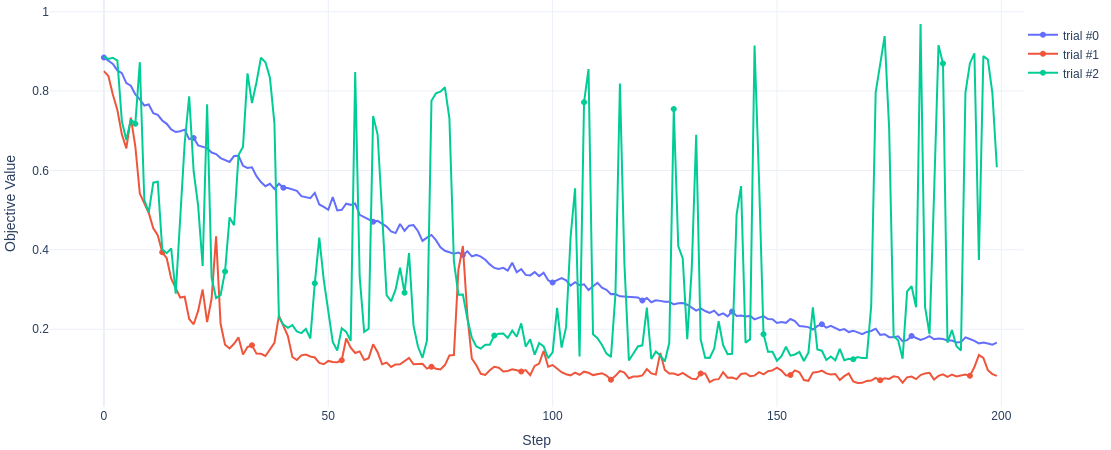
\includegraphics[width=1\linewidth]{PICTURES/loss_None.png} 
    \caption{Validation loss values for three different learning rates over 200 epochs.} \label{fig:loss-None} 
\end{figure}

Next, the main optimization was conducted using the linear scheduler and the best values from the previous step. The hyperparameters discussed in section \ref{sec:1.2.8} were optimized, resulting in 18 combinations (2 * 3 * 3 = 18). The complete results are shown in Table~\ref{tab:main_results}, ordered from lowest to highest validation loss, with the best result appearing at index 8.
\begin{table}[H]
    \centering
    \caption{Validation loss and corresponding hyperparameters across trials}
    \renewcommand{\arraystretch}{1.1}

    \begin{tabular}{ccccc}
        \toprule
        \textbf{Idx} & \textbf{Val Loss} & \textbf{Depth} & \textbf{Filters} & \textbf{Patch Size} \\
        \midrule
        15 & 0.0657 & 5 & 16 & 128 \\
        4  & 0.0643 & 3 & 8  & 128 \\
        0  & 0.0643 & 5 & 8  & 128 \\
        7  & 0.0636 & 4 & 8  & 128 \\
        2  & 0.0631 & 5 & 32 & 128 \\
        9  & 0.0601 & 4 & 16 & 128 \\
        10 & 0.0600 & 3 & 32 & 128 \\
        5  & 0.0574 & 4 & 32 & 128 \\
        11 & 0.0573 & 3 & 16 & 128 \\
        6  & 0.0444 & 5 & 8  & 256 \\
        12 & 0.0427 & 3 & 8  & 256 \\
        13 & 0.0424 & 4 & 8  & 256 \\
        16 & 0.0407 & 5 & 16 & 256 \\
        3  & 0.0401 & 3 & 16 & 256 \\
        17 & 0.0401 & 4 & 16 & 256 \\
        14 & 0.0392 & 5 & 32 & 256 \\
        8  & 0.0389 & 3 & 32 & 256 \\
        \textbf{1}  & \textbf{0.0382} & \textbf{4} & \textbf{32} & \textbf{256} \\

        \bottomrule
    \end{tabular}
    \label{tab:main_results}
\end{table}


Figure \ref{fig:validation_loss} presents the validation loss for the best (trial 1) and worst (trial 15) values over 200 epochs. The plot shows that both losses decrease rapidly during the first 50 epochs, after which they oscillate around the same value. Despite this, trial 1 achieves a lower minimum loss compared to trial 15.

\begin{figure}[H]
    \centering
    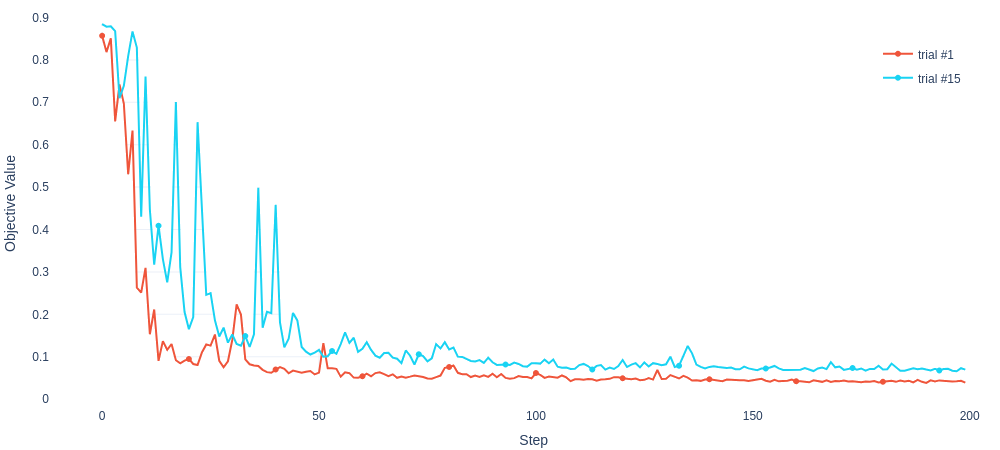
\includegraphics[width=0.75\linewidth]{PICTURES/loss.png}
    \caption{Validation loss over 200 epochs}
    \label{fig:validation_loss}
\end{figure}


Figure~\ref{fig:Hyperparameter-Importance} shows the importance of each hyperparameter, providing valuable insights into the model training process. As shown in Table~\ref{tab:main_results}, larger patch sizes and a higher number of start filters tend to achieve better results compared to smaller ones. This explains why their importance is higher than that of the model depth, as they have a greater influence on the final loss value.
\begin{figure}[H]
    \centering
    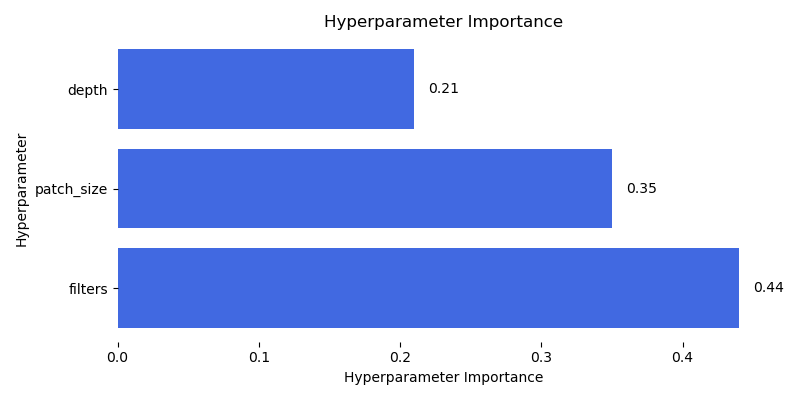
\includegraphics[width=0.75\linewidth]{PICTURES/hyperparam.png}
    \caption{Hyperparameter importance}
    \label{fig:}
\end{figure}

The final two runs were conducted using the best hyperparameters, but with datasets that included labels generated by polygons and K-means clustering. The models with the best validation losses were chosen. 
%The corresponding validation loss values are presented in Table \ref{tab:val_loss_values}.
%\begin{table}[H]
%    \centering
%    \caption{Validation loss values for different labeling methods}
%    \renewcommand{\arraystretch}{1}
    
%    \begin{tabular}{lccc}
%        \toprule
%        \textbf{Metric} & \textbf{K-means Refined} & \textbf{K-means} & \textbf{Polygon} \\
%        \midrule
%        Validation Loss & 0.02892 & 0.03118 & 0.09698 \\
%        \bottomrule
%    \end{tabular}
%    \label{tab:val_loss_values}
%\end{table}
%

Since both validation sets use labels derived from their respective training sets, the resulting performance metrics may not be fully reliable. A more meaningful assessment can be made by evaluating the model on unseen test images using labels generated through refined K-means clustering. Although neither the K-means nor polygon labels are intended for use in this final workflow, this evaluation can provide insight into whether either labeling method is sufficient for future training.



\subsection{Evaluation on Test Data}

Three primary evaluation metrics were used:

\begin{itemize} 
\item \textbf{Mean IoU}: The intersection over union (IoU) is calculated and averaged across all test data. 
\item \textbf{Min IoU}: The minimum IoU value is used to assess the worst-case scenario. 
\item \textbf{Mean Hausdorff Distance}: Measures the average greatest distance across all test images. 
\item \textbf{Max Hausdorff Distance}: Represents the maximum of these distances, giving an indication of the worst mismatch in a picture. \end{itemize}

\subsubsection{Evaluation metrics}

The IoU metric is calculated as shown in Equation ~\ref{eq:iou_smooth}, without the transformation $1 - \text{IoU}$, meaning that a higher IoU indicates better results.

\subsubsection{Hausdorff Distance}

The Hausdorff distance~\cite{henrikson1999completeness} (HD) quantifies how far two shapes (or point sets) are from each other. It is defined as the greatest of all the distances from a point in one set to the nearest point in the other set, as is shown in Figure ~\ref{fig:hausdorff}. In essence, it captures the largest error between the two sets, highlighting the worst-case mismatch.
\begin{figure}[H]
    \centering
    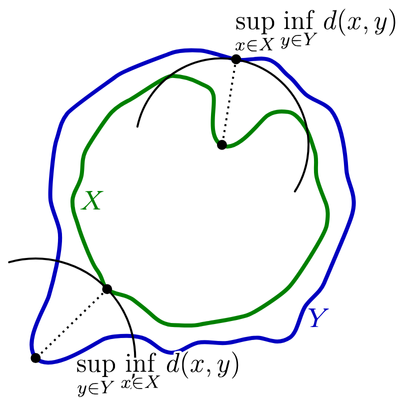
\includegraphics[width=0.45\textwidth]{PICTURES/haussdorf.png}
    \caption{Visualization of Hausdorff distance between two shapes. The dotted line represent the closest-point distances from one shape to the other; the longer dotted line determines the Hausdorff distance.\cite{wikipediaHausdorff}}
    \label{fig:hausdorff}
\end{figure}

Mathematically, there are two sets of points $A$ and $B$, the Hausdorff distance $d_H(A, B)$ is defined as:

\begin{equation}
d_H(A, B) = \max\left\{ \sup_{a \in A} \inf_{b \in B} \|a - b\|,\; \sup_{b \in B} \inf_{a \in A} \|b - a\| \right\}
\label{eq:hausdorff}
\end{equation}
In this equation:
\begin{itemize}
    \item \( \|a - b\| \) is the Euclidean distance between a point \( a \in A \) and a point \( b \in B \).
    \item \( \inf_{b \in B} \|a - b\| \) is the \textbf{infimum} (i.e., the greatest lower bound), which in this context corresponds to the minimum distance from point \( a \) in set \( A \) to any point in set \( B \).
    \item \( \sup_{a \in A} (\cdot) \) is the \textbf{supremum} (i.e., the least upper bound), which corresponds to the maximum of those minimum distances over all points in \( A \).
\end{itemize}

The Hausdorff distance computes the maximum of two distances:
\begin{enumerate}
    \item The greatest of all shortest distances from a point in \( A \) to the set \( B \).
    \item The greatest of all shortest distances from a point in \( B \) to the set \( A \).
\end{enumerate}



This metric is symmetric and measures the maximum distance from a point on one shape to the closest point on the other shape, making it highly sensitive to outliers. 

\subsubsection{Results}
The evaluation results are presented in Table \ref{tab:test_results}:

\begin{table}[H]
    \centering
    \caption{Evaluation Results on Test Data}
    \renewcommand{\arraystretch}{1.2}
    
    \begin{tabular}{lccc}
        \toprule
        \textbf{Metric} & \textbf{K-means Refined} & \textbf{K-means} & \textbf{Polygon} \\
        \midrule
        Mean IoU & 0.95155 & 0.84833 & 0.89800 \\
        Min IoU  & 0.64854 & 0.18043 & 0.72229 \\
        Mean HD  & 53.83457 & 75.51385 & 91.68906 \\
        Max HD  & 284.51977 & 288.06249 & 337.45242 \\
        \bottomrule
    \end{tabular}
    \label{tab:test_results}
\end{table}


The results reveal some key patterns. The model trained with polygon labels performed surprisingly well, with good overall IoU, although the Hausdorff Distance (HD) was relatively poor. On the other hand, the model trained with K-means labels achieved the lowest IoU values. This could be explained by the fact that the K-means labels didn't differentiate well enough between oxidation and coating areas, leading to poorer segmentation. The figure~\ref{fig:comparison} highlights the comparison of the three types of predictions made by models trained with different kinds of labels, alongside the original ground truth label, on a particularly complex sample. The best results across all four metrics were achieved with the K-means refined labels, as expected.


Figure \ref{fig:kmeans} illustrates that the model trained with K-means labels struggles to differentiate between the oxidation and coating layers, leading to poor performance. In contrast, Figures \ref{fig:polygon} and \ref{fig:kmeans-refined} show that the models trained on polygonal and K-means refined labels can accurately predict the coating layers, despite the complexity of the images and the challenge of distinguishing between the layers. However, Figure \ref{fig:polygon} still struggles with finer details, particularly at the boundaries of the layers.


\begin{figure}[H]
    \centering
    \begin{subfigure}[b]{0.75\linewidth}
        \centering
        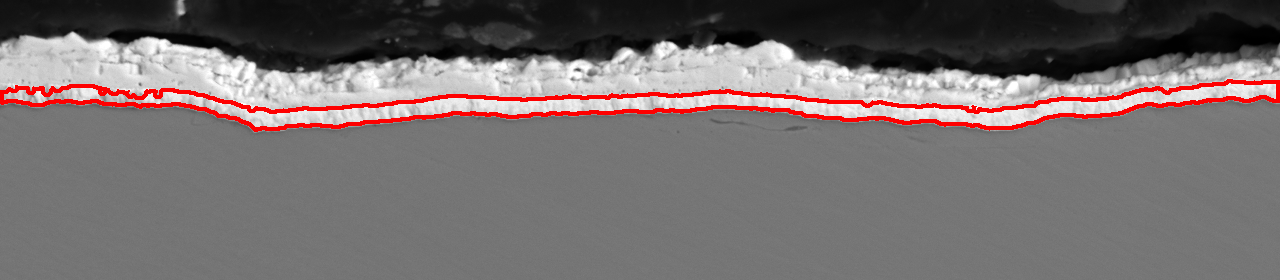
\includegraphics[width=\linewidth]{PICTURES/eval/188_kmeans_refined.png}
        \caption{K-means refined label prediction}
        \label{fig:kmeans-refined}
    \end{subfigure}
    
    \vspace{0.5cm}
    
    \begin{subfigure}[b]{0.75\linewidth}
        \centering
        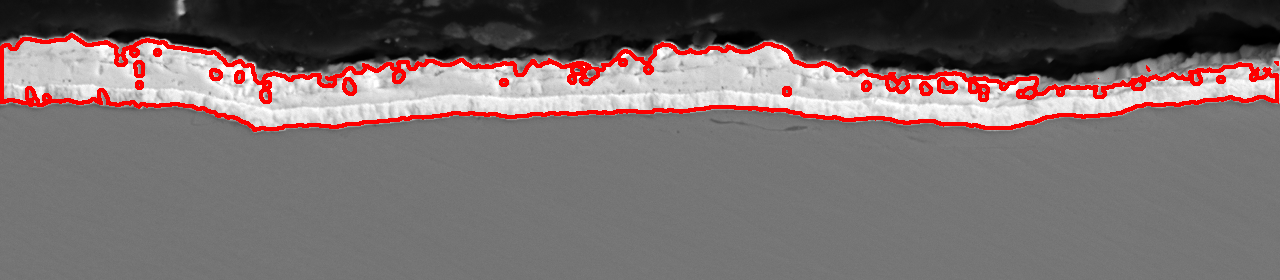
\includegraphics[width=\linewidth]{PICTURES/eval/188_kmeans.png}
        \caption{K-means label prediction}
        \label{fig:kmeans}
    \end{subfigure}

    \vspace{0.5cm}
    
    \begin{subfigure}[b]{0.75\linewidth}
        \centering
        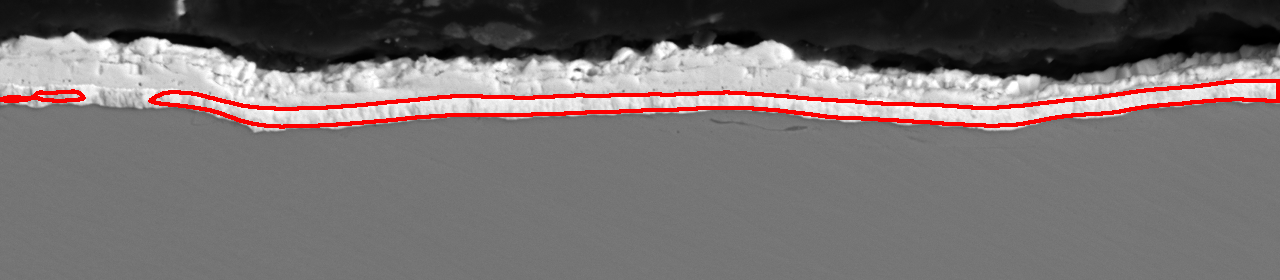
\includegraphics[width=\linewidth]{PICTURES/eval/188_polygon.png}
        \caption{Polygon label prediction}
        \label{fig:polygon}
    \end{subfigure}
    
    \vspace{0.5cm}
    
    \begin{subfigure}[b]{0.75\linewidth}
        \centering
        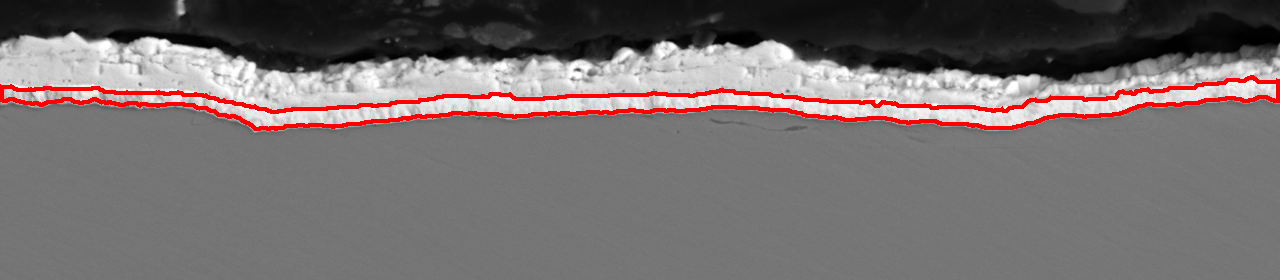
\includegraphics[width=\linewidth]{PICTURES/eval/188_og.png}
        \caption{Original label}
        \label{fig:ground-truth}
    \end{subfigure}
    
    \caption{Comparison of predictions made by models trained on different labels, alongside the original ground truth label on a complex sample.}
    \label{fig:comparison}
\end{figure}




To highlight the superiority of the U-Net model over the K-means algorithm in segmenting the image, it is important to note that the K-means method struggled to distinguish between the oxidation layer and the coating layer, as shown in Figure~\ref{fig:kmean_sem_color}. In contrast, as shown in Figure~\ref{fig:149}, the model trained on the K-means refined labels was able to successfully learn this pattern.

\begin{figure}[H] 
\centering 
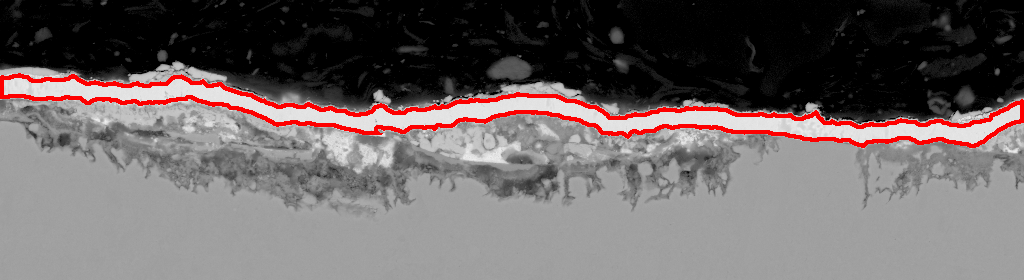
\includegraphics[width=0.8\linewidth]{PICTURES/eval/149(1).png} 
\caption{Prediction labels shown in red border on the original image with extensive oxidation} \label{fig:149} \end{figure}

An important part of the evaluation is also to inspect the images that caused the minimum IoU and Hausdorff Distance (HD). The lowest IoU occurred on an image with the thinnest coating layer in the entire training or testing dataset, as can be seen in Figure~\ref{fig:min_iou}. This highlights the need for a more robust and heterogeneous dataset, as small datasets, like the one used here, can lead to issues where less frequent or extreme cases—such as images with very thin coatings—cause problems during model evaluation.

 \begin{figure} [H]
    \centering 
    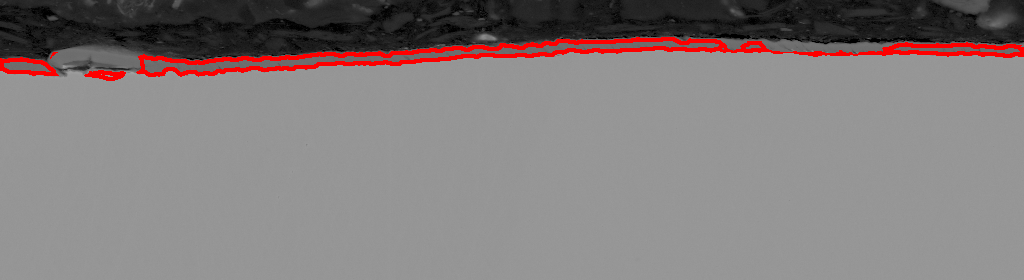
\includegraphics[width=0.70\linewidth]{PICTURES/eval/66.png} \caption{Example image with minimum IoU} \label{fig:min_iou}
 \end{figure}
On the other hand, the lowest HD was observed on an image containing a dark defect located at the bottom, as shown in Figure~\ref{fig:max_hd}. However, this deviation is not particularly concerning, as such anomalies can be effectively addressed with simple postprocessing steps. These types of deviations are relatively easy to detect and remove.
 \begin{figure}[H]
        \centering
        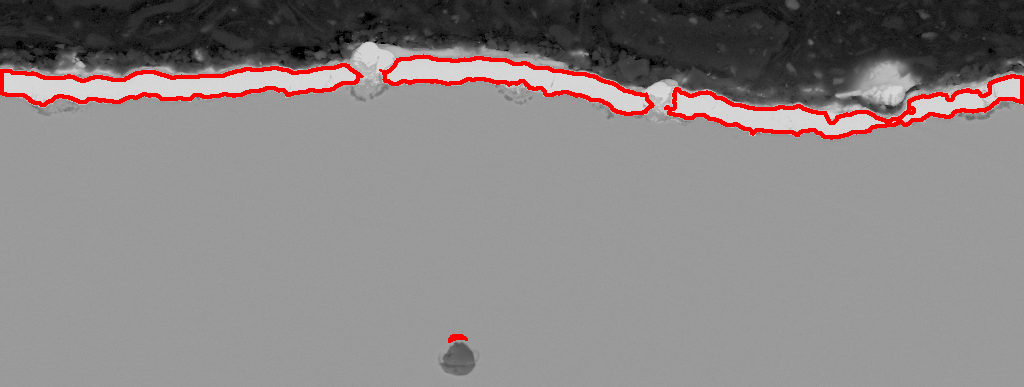
\includegraphics[width=0.65\linewidth]{PICTURES/eval/113.png}
        \caption{Example image with maximum HD}
        \label{fig:max_hd}
    \end{figure}


